\documentclass{report}
\usepackage{titling} % For subtitle
\usepackage{tocloft} % For customizing TOC formatting
\usepackage{soul} % For highlighting text
\usepackage{xcolor}
\usepackage{graphicx}


% Manually setting the margins
\setlength{\textwidth}{\dimexpr 15.4cm}  % Width of text area
\setlength{\textheight}{\dimexpr 23.4cm} % Height of text area
\setlength{\oddsidemargin}{-0.25in}      % Left margin (negative value reduces margin)
\setlength{\evensidemargin}{-0.25in}     % Even page left margin (for two-sided printing)
\setlength{\topmargin}{-0.5in}           % Top margin
\setlength{\headheight}{14pt}            % Space for header (optional)
\setlength{\headsep}{25pt}               % Space between header and text
\setlength{\footskip}{30pt}              % Distance from bottom of text to footer

% Set the main font to Helvetica
\usepackage[scaled]{helvet}
\renewcommand{\rmdefault}{phv}

% Set highlight colour
\sethlcolor{yellow}

\begin{document}

% Title Page Formatting
\title{MSc in Computing - Team Project}
\title{User Evaluation Report - Magpie (Group 3)}
\author{Anais Blenet\\Saul Burgess\\Yuanshuo Du\\Jessica Fornetti\\Andreas Kraus}
\date{\today}

% Customizing TOC formatting
\renewcommand{\cfttoctitlefont}{\hfill\Huge\bfseries} % Center TOC title
\renewcommand{\cftaftertoctitle}{\hfill}

\maketitle % Generates the title page

% Table of Contents
\tableofcontents
\newpage

% Main Body
\chapter{Introduction}
\section{Proposed Hypothesis}
Our project's goal is to provide a easy-to-use Geographical Information Service
in county Dublin. In our preliminary research, we couldn’t find a singular
system that allowed users to gain a general overview of public amenities, for
example, parking, bike infrastructure, or public transport. In Ireland and the
United Kingdom, the prevalence of proper digitised records in county
administrations varies wildly (Lynn et al., 2023). Some make use of
state-of-the-art geographical information systems (GIS) while others rely on
spreadsheets which are manually kept up to date. (McGuirk and MacLaran, 2001) A
system that would allow users to quickly inspect a combined dataset grounded in
automatically generated, real-world data could accelerate processes like
planning permissions, urban development, or resource allocation.\\ \\
Prior to user evaluation, exploratory work was conducted in the forms of a
market research survey to answer key demographic \& product questions:
\begin{enumerate}
    \item Who is our primary target user?
    \item What kind of amenity data do they access and how?
    \item What devices/tools do they primarily use?
    \item Are they satisfied with those tools?
    \item Would they consider Magpie useful in filling the gaps in their
          toolset?
\end{enumerate}
Responses from the survey further allowed us to confirm our target demographic
(figure 1.1), find out the proportion of users using amenity data for their work
(figure 1.2), what type of amenity data  they require access to (figure 1.3) and
why current tools are unsatisfactory (figure 1.4).
\begin{figure}
    \centering
    \begin{minipage}{0.45\textwidth}
        \centering
        \fbox{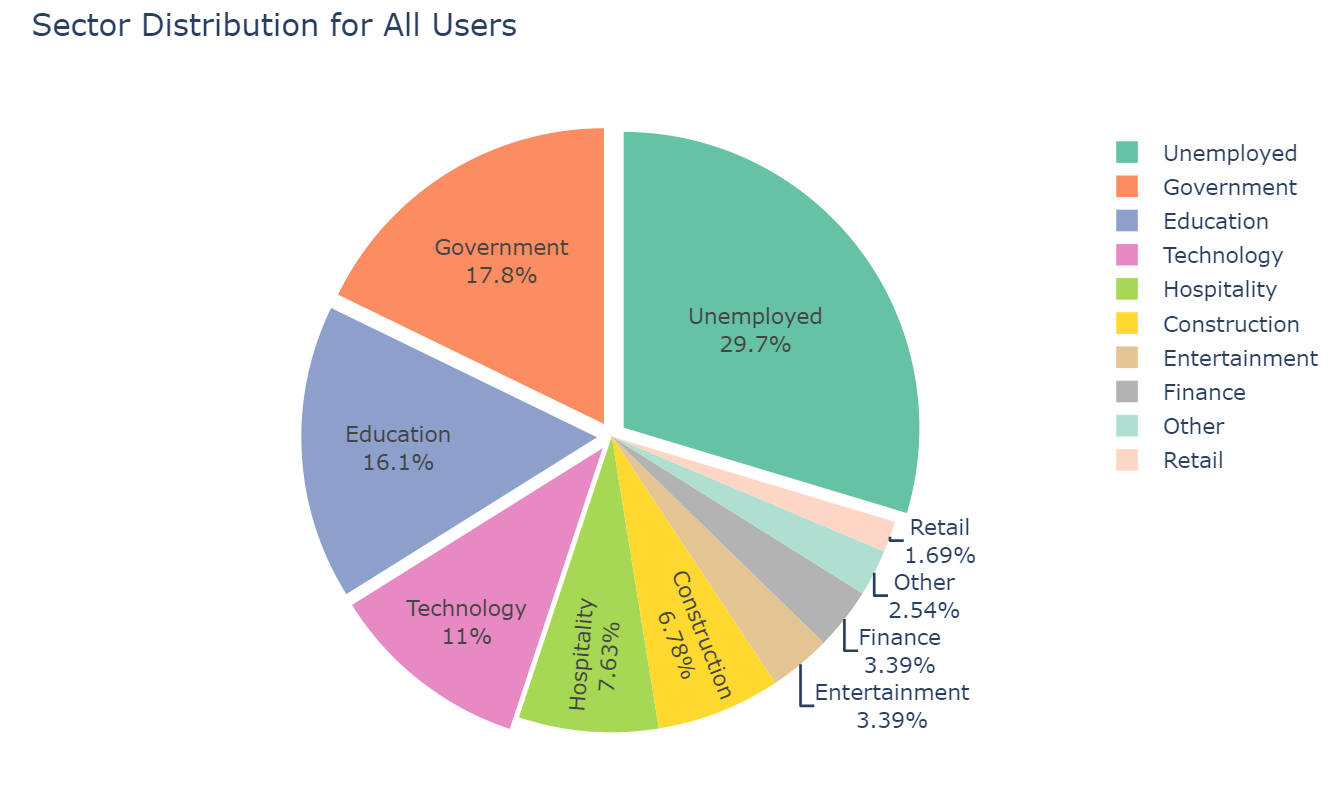
\includegraphics[width=\textwidth]{Figures/fig1.png}}
        \caption{Target user sectors}
        \label{fig:plot1}
    \end{minipage}
    \hfill
    \begin{minipage}{0.45\textwidth}
        \centering
        \fbox{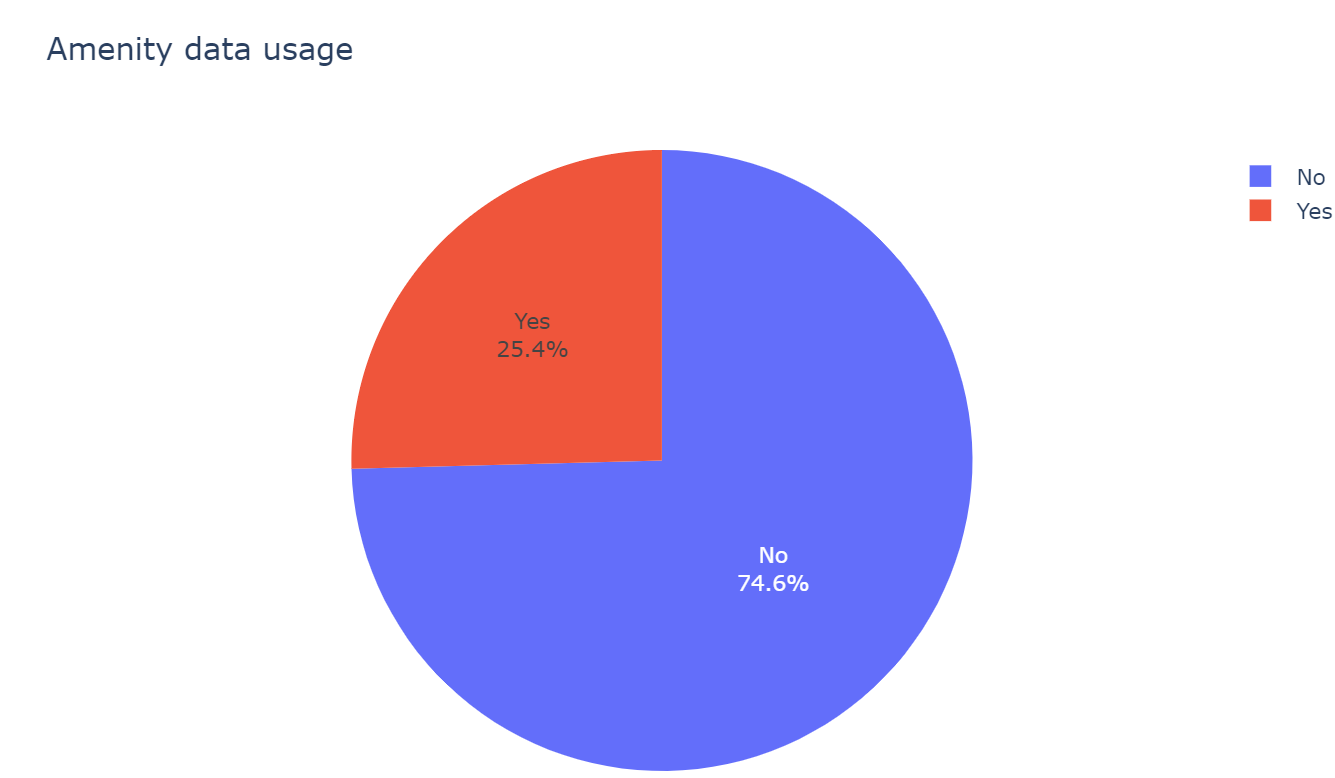
\includegraphics[width=\textwidth]{Figures/fig2.png}}
        \caption{Amenity Access distribution}
        \label{fig:plot2}
    \end{minipage}
\end{figure}
These responses also cemented the need of Magpie (figure 1.5) for both casual
users (User A) \& professionals who require amenity data (User B).
\begin{figure}
    \centering
    \begin{minipage}{0.5\textwidth}
        \centering
        \fbox{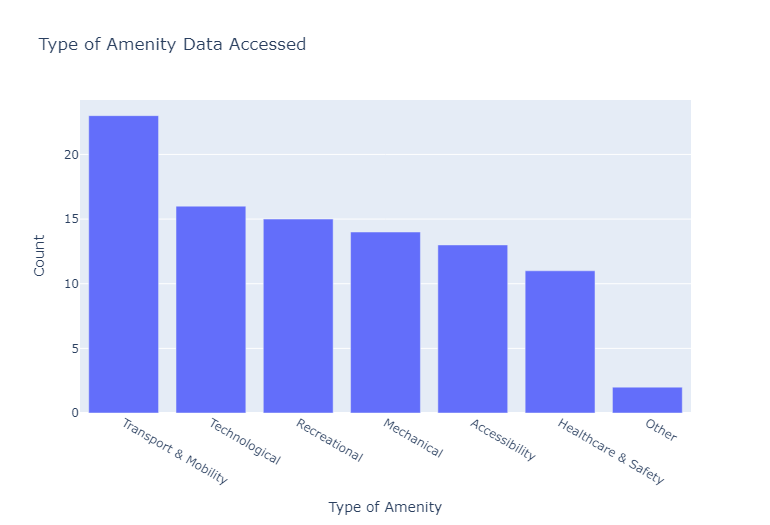
\includegraphics[width=\textwidth]{Figures/fig3.png}}
        \caption{Current amenity data accessed}
        \label{fig:plot3}
    \end{minipage}
    \hfill
    \begin{minipage}{0.6\textwidth}
        \centering
        \fbox{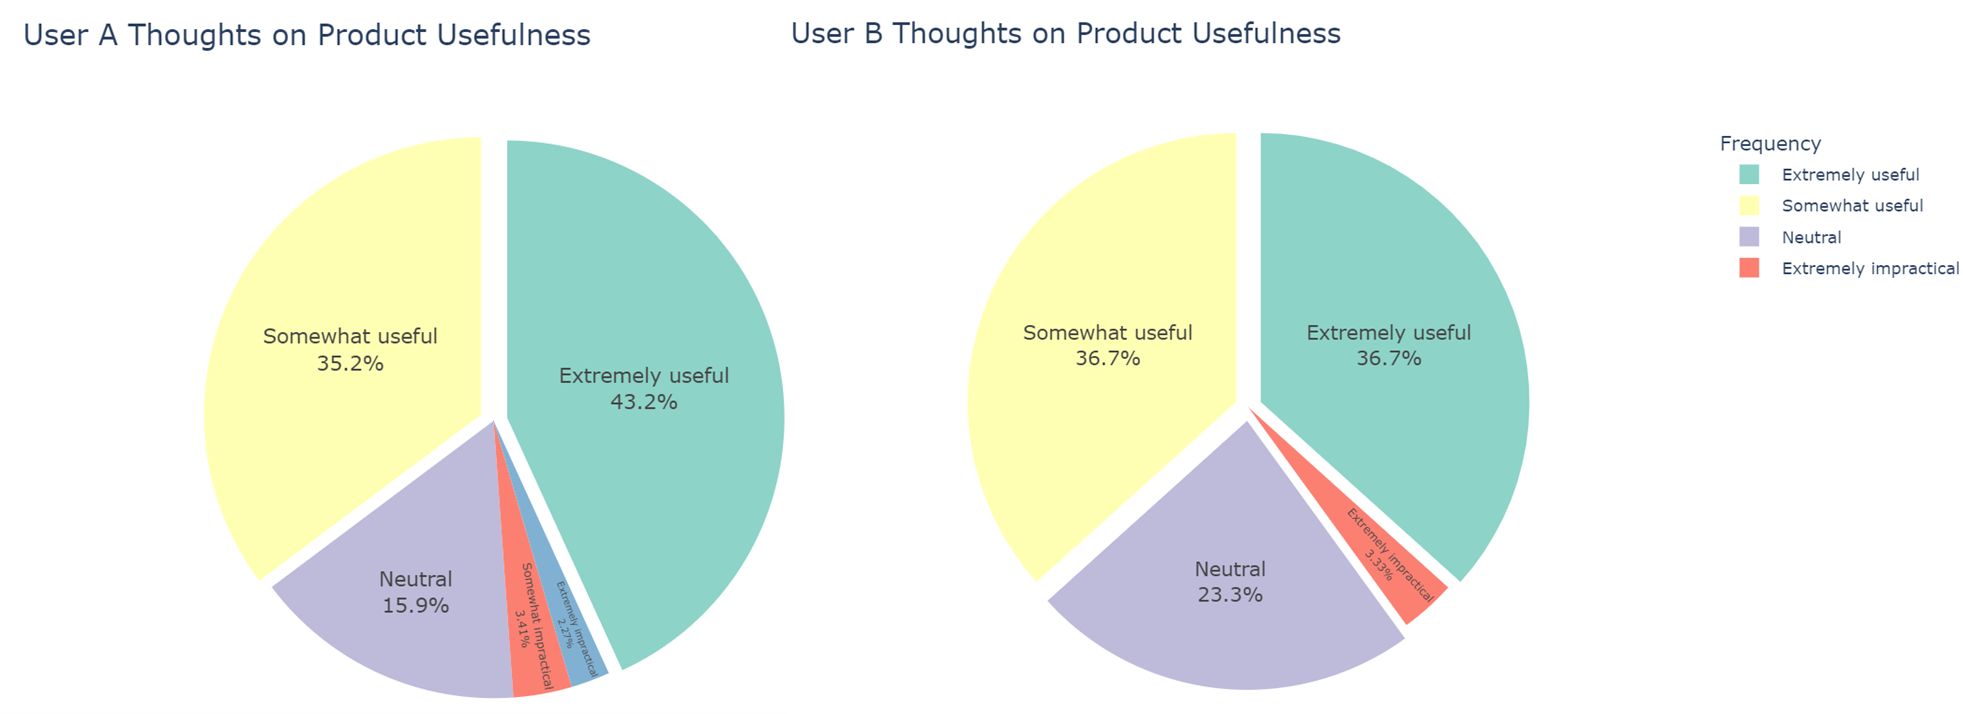
\includegraphics[width=\textwidth]{Figures/fig4.png}}
        \caption{Current tools \& satisfaction rate}
        \label{fig:plot4}
    \end{minipage}
    \hfill
    \begin{minipage}{0.6\textwidth}
        \centering
        \fbox{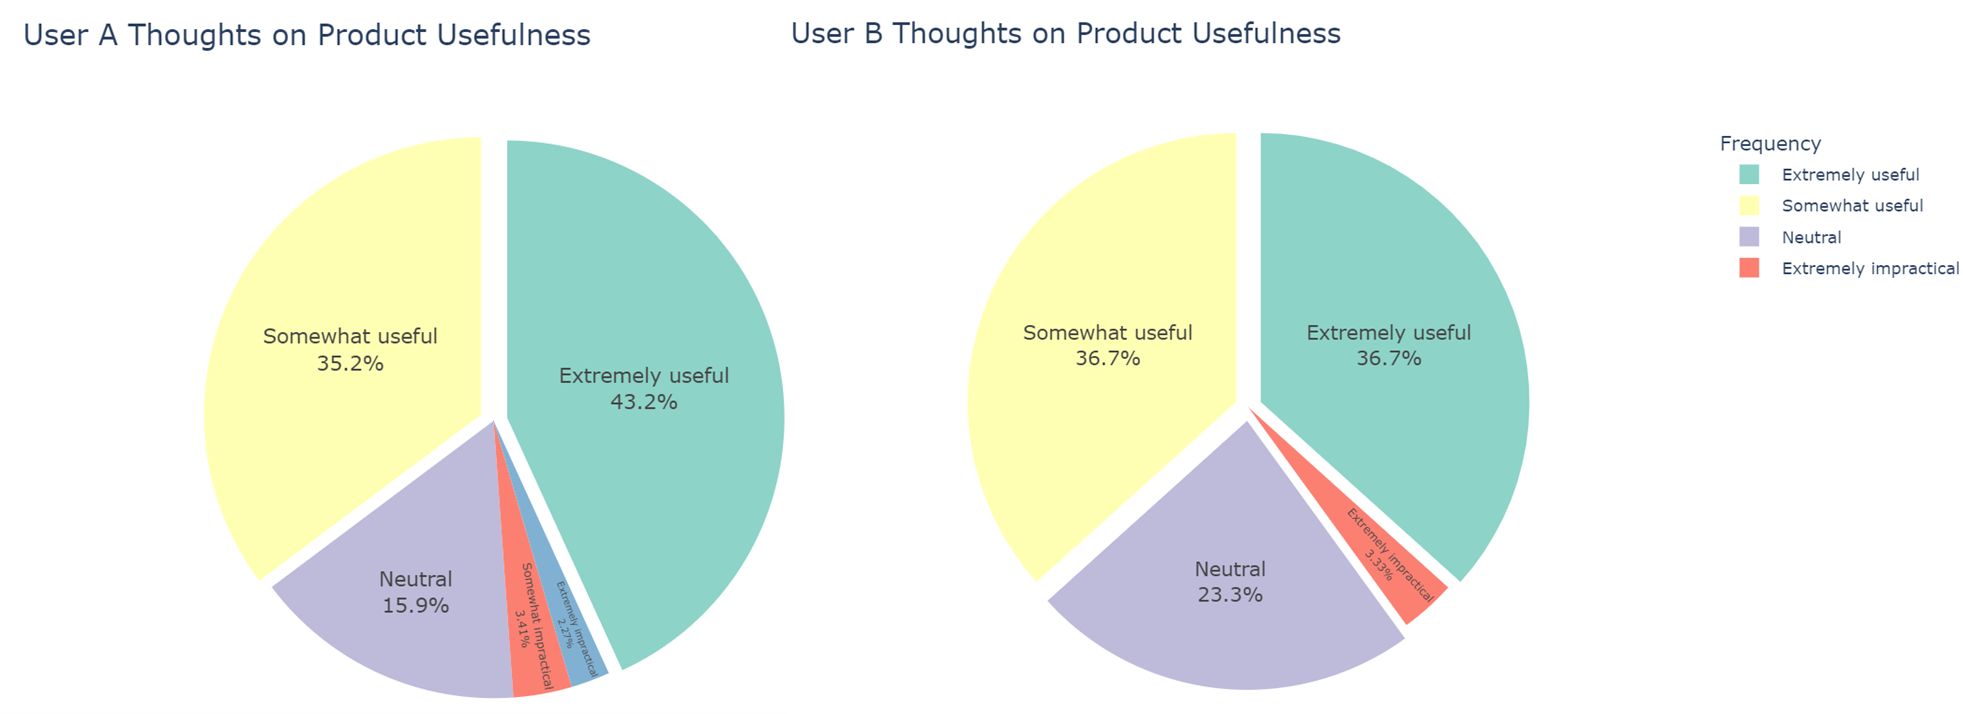
\includegraphics[width=\textwidth]{Figures/fig5.png}}
        \caption{Magpie potential}
        \label{fig:plot5}
    \end{minipage}
\end{figure}

\noindent{}The survey also helped us implement additional features (figure
1.6,1.7 \& 1.8) prior to the user evaluation such as a dashboard with search
functionality and filters.\\ \\

\begin{figure}
    \centering
    \begin{minipage}{0.45\textwidth}
        \centering
        \fbox{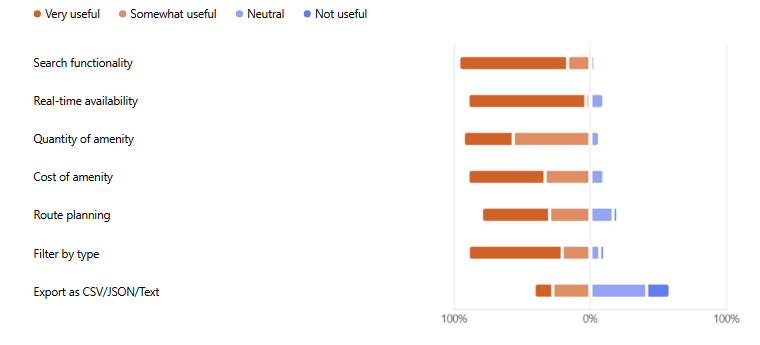
\includegraphics[width=\textwidth]{Figures/fig6.png}}
        \caption{Additional features rating}
        \label{fig:plot6}
    \end{minipage}
    \hfill
    \begin{minipage}{0.45\textwidth}
        \centering
        \fbox{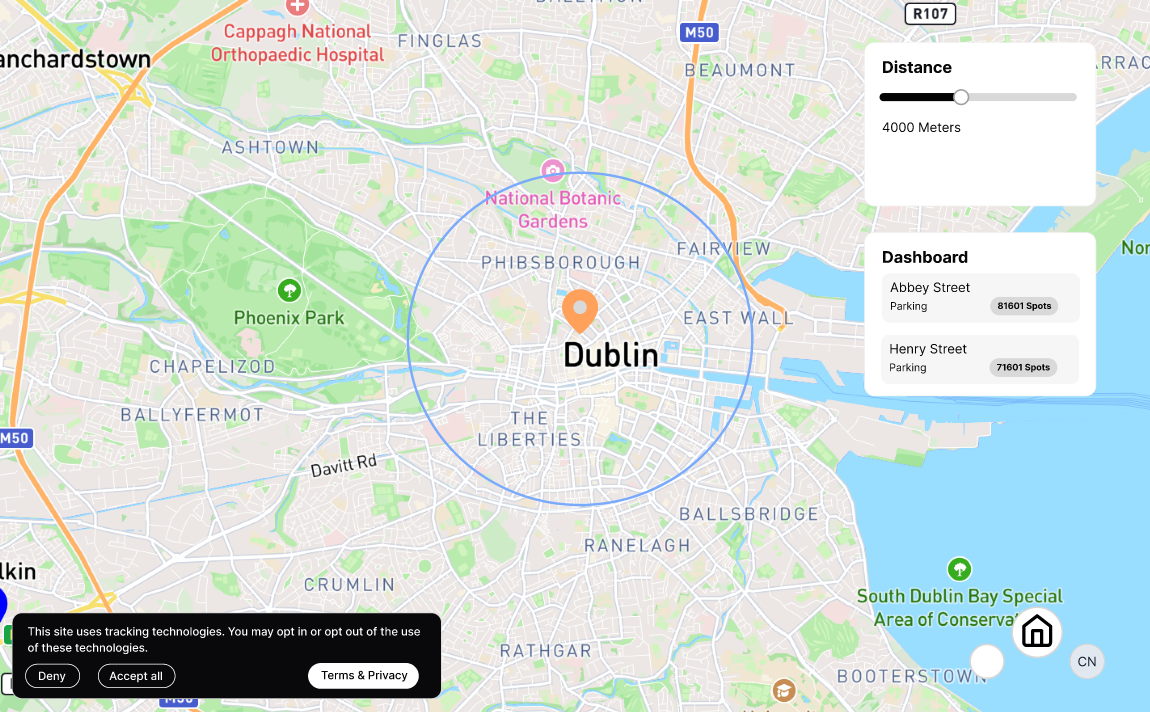
\includegraphics[width=\textwidth]{Figures/fig7.png}}
        \caption{Version 1 of high fidelity prototype}
        \label{fig:plot7}
    \end{minipage}
    \hfill
    \begin{minipage}{0.45\textwidth}
        \centering
        \fbox{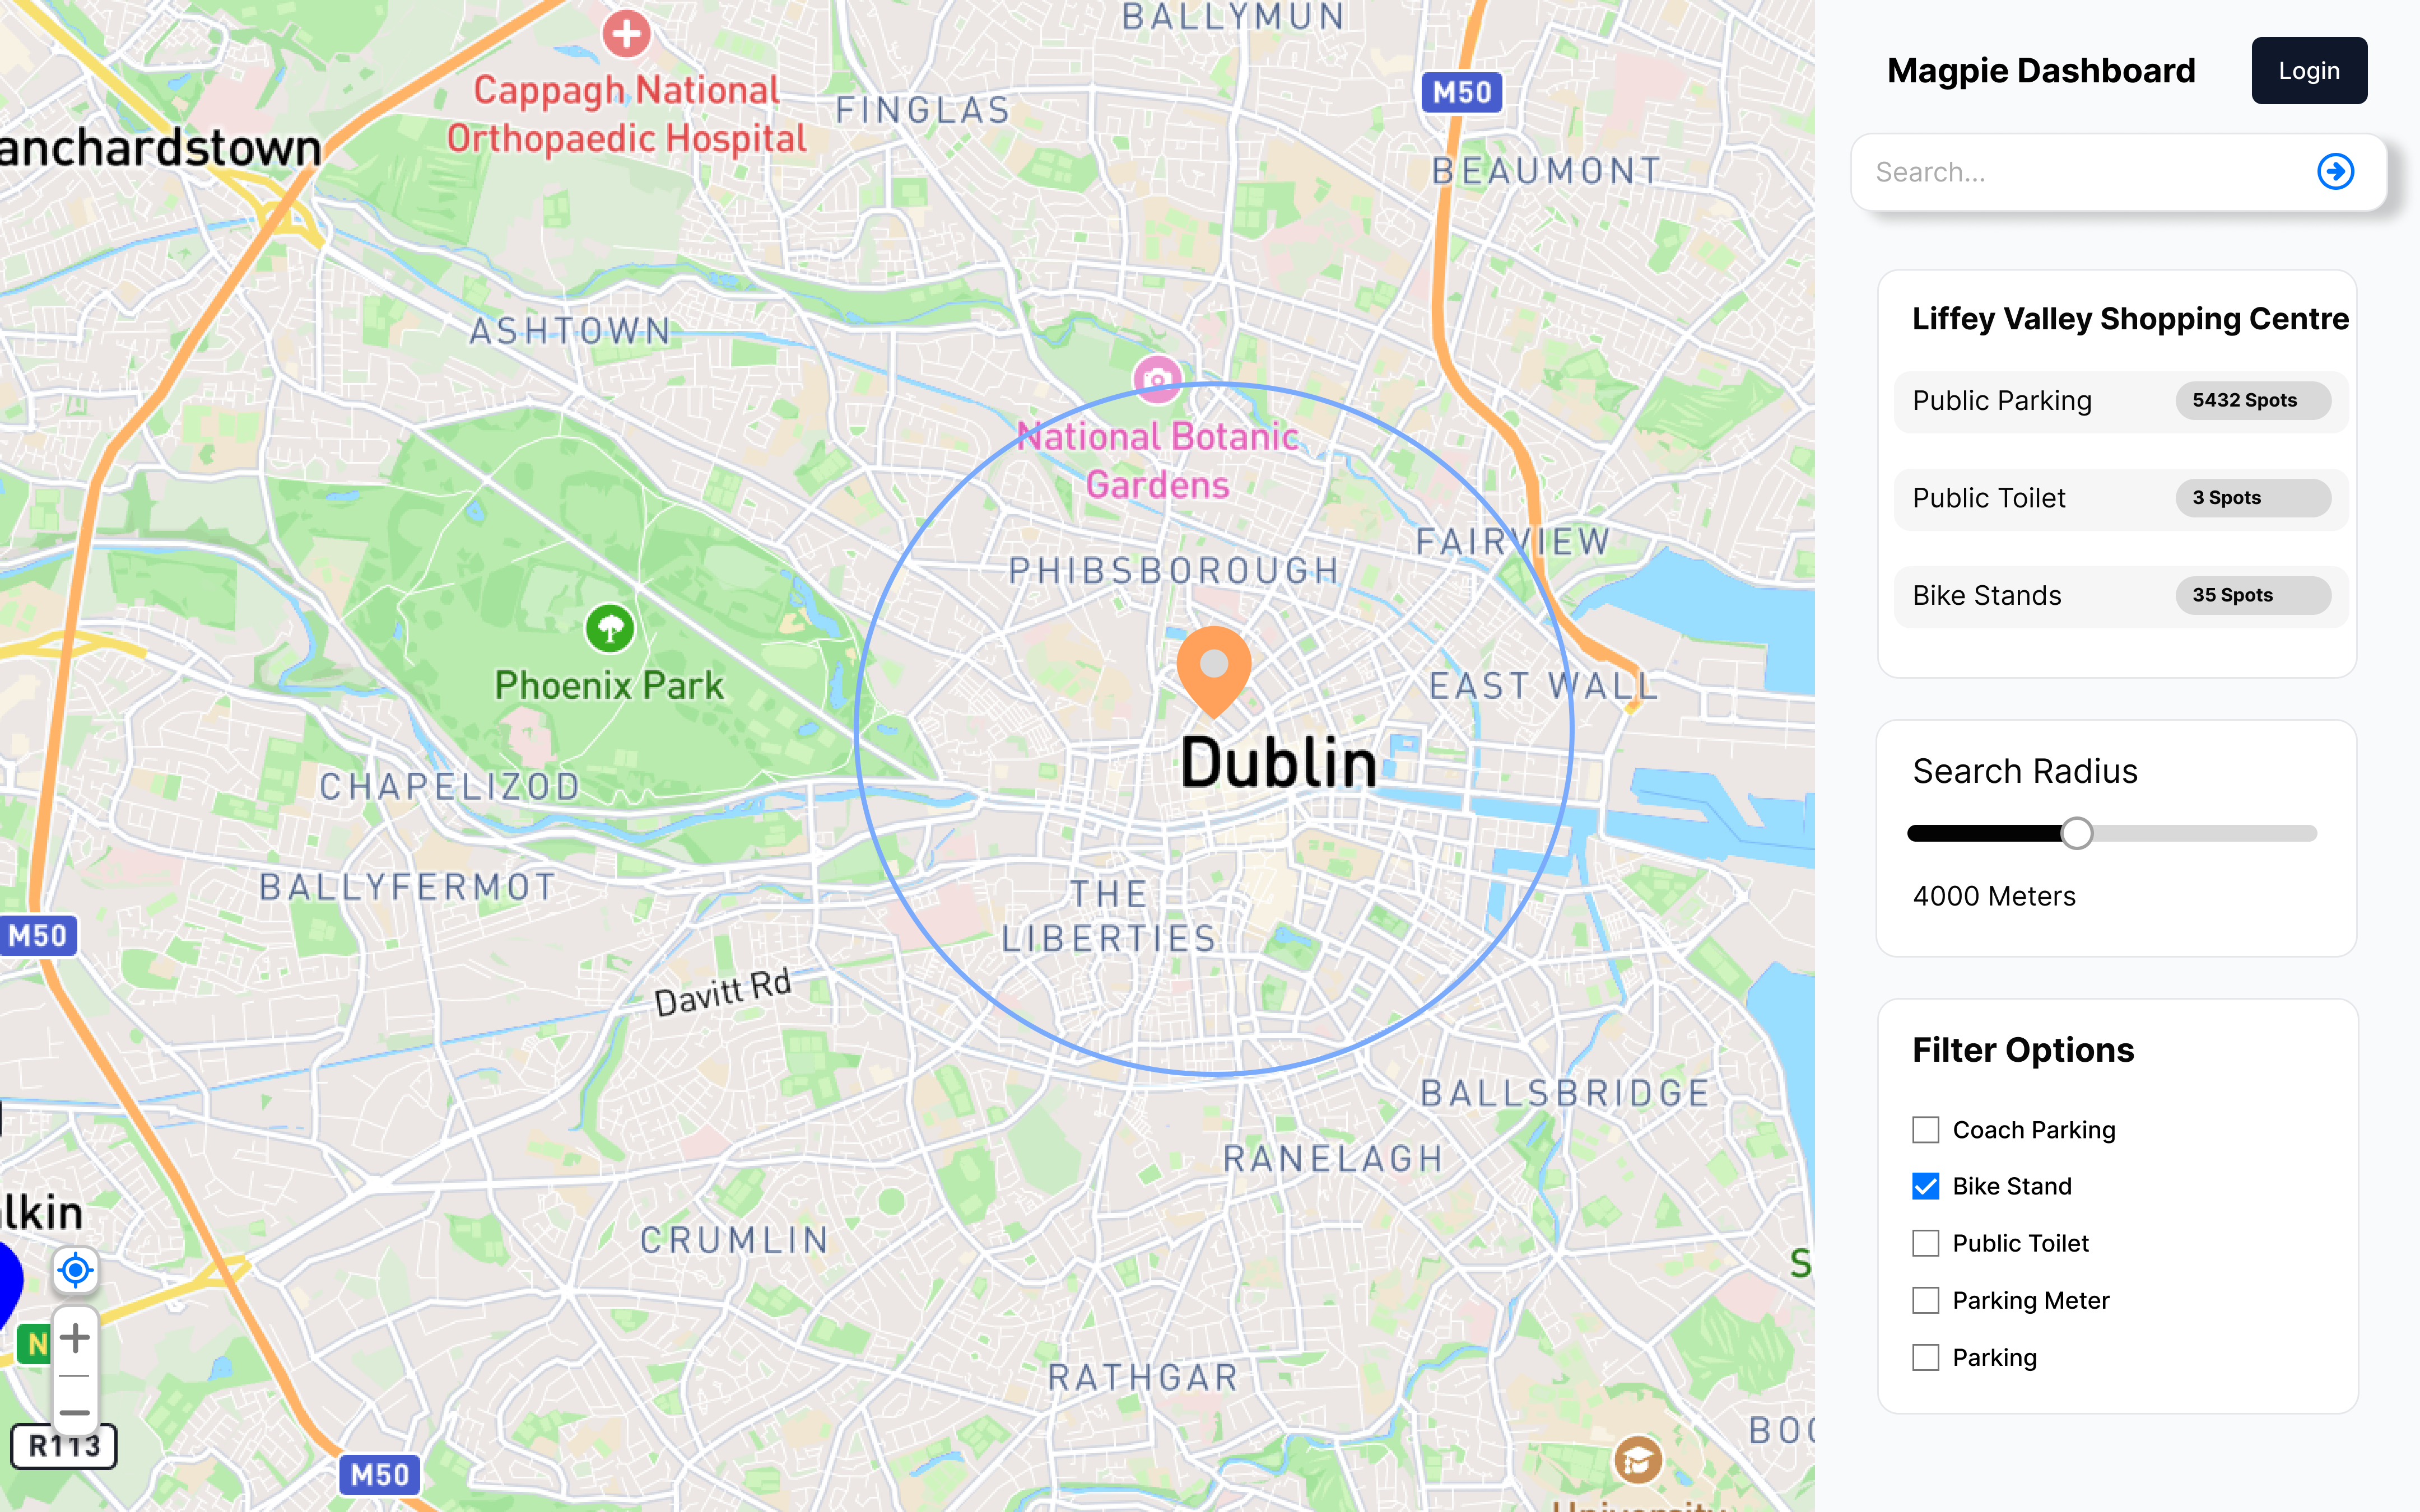
\includegraphics[width=\textwidth]{Figures/fig8.png}}
        \caption{Version 2 of high-fidelity prototype}
        \label{fig:plot8}
    \end{minipage}
\end{figure}

\noindent{}Magpie has remedied the first challenge of fragmented information on
amenities, and through this user evaluation, we hope to address the second challenge
which is making the access to this information easy, quick \& accessible.

\chapter{Experimental Methods}
The goal of the user evaluation is to gain feedback from real users, learn if
Magpie works as expected and assess how user-friendly it is. We will be using 2
main methods to collect both qualitative data through open-ended questions, and
quantitative data from multiple choice questions from which we will derive
insights to improve the Magpie user experience.
\section{Usability Testing}
\subsection{Casual feedback}
\begin{enumerate}
    \item \underline{Objective:} Obtain quick feedback through frontend development process to implement features of the Minimum Viable Product
    \item \underline{Conditions:} Oral feedback, written notes
    \item \underline{Methodology:} Asking for feedback from users in the immediate circle on a certain new feature/process/item of Magpie application, their experience interacting with it and what they would prefer/or not instead.
    \item \underline{Baseline \& Evaluation metrics:} No baseline; user experience is evaluated casually. This method serves as the "Step 0" of usability testing in helping us implement "Draft 1" of new features.
\end{enumerate}
\subsection{Uncontrolled (Remote)}
\begin{enumerate}
    \item \underline{Objective:} Evaluate user experience in an uncontrolled
          environment, assess overall functioning of Magpie \& identify any
          potentional usability issues
    \item \underline{Conditions:} Online followed up by survey
    \item \underline{Methodology:} Share the link to Magpie online through the same channels we used for the market research survey, ask them to participate in testing Magpie freehanded.
    \item \underline{Baseline \& Evaluation metrics:} No baseline; user experience will be evaluated through a satisfaction survey (figure 2.1).
\end{enumerate}
\begin{figure}
    \begin{minipage}{\textwidth}
        \centering
        \fbox{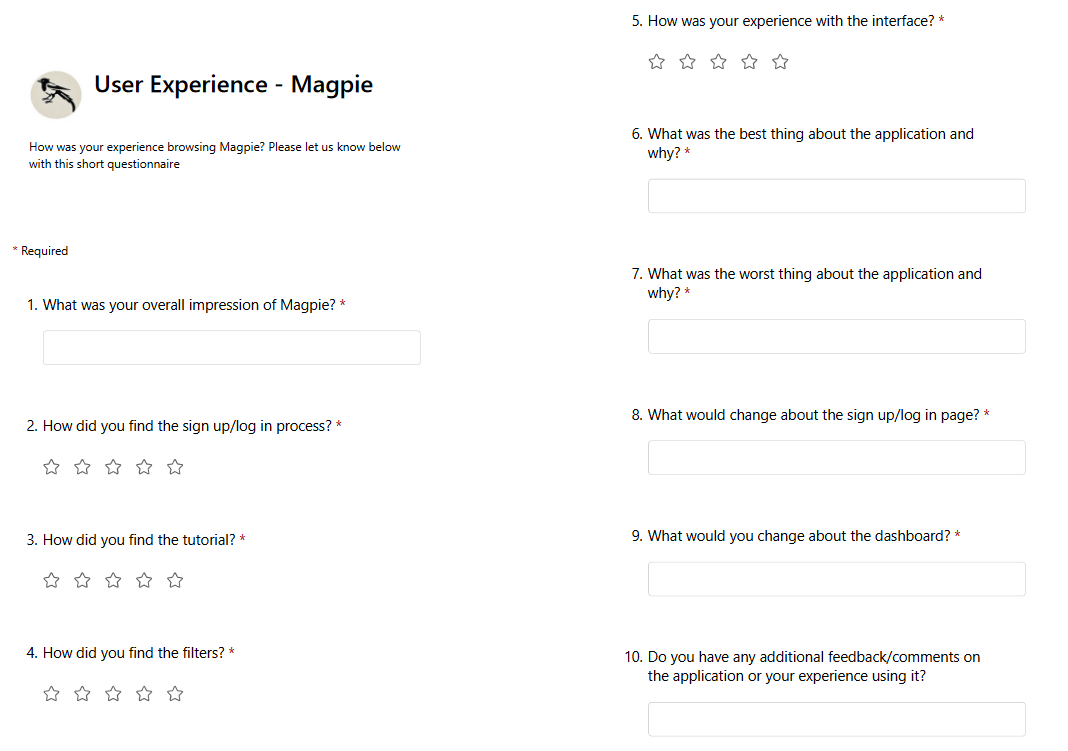
\includegraphics[width=\textwidth]{Figures/fig9.png}}
        \caption{User experience survey}
        \label{fig:plot9}
    \end{minipage}
\end{figure}
\subsection{Controlled (Remote)}
\begin{enumerate}
    \item \underline{Objective:} Analyze how users interact with Magpie in a
          controlled environment guided by specific instructions and tasks to complete
          \& identify any potentional usability issues
    \item \underline{Conditions:} Online through remote usability tools
          (SessionReplay/Contentsquare)
    \item \underline{Methodology:} Reach out to casual users who left their contact
          email in the market research survey, propose for them to participate in user
          evaluation survey, conduct the experiment, \hl{bla bla bla}.
    \item \underline{Baseline \& Evaluation metrics:} No baseline; user
          experience will be evaluated on rate of completion of tasks, difficulties
          encountered when completing tasks
\end{enumerate}
\subsection{Field test (Remote)}
\begin{enumerate}
    \item \underline{Objective:} Analyze how users interact with Magpie in a
          controlled environment guided by their own tasks for their day-to-day work
          \& identify any potentional usability issues
    \item \underline{Conditions:} Online through remote usability tools
          (SessionReplay/Contentsquare)
    \item \underline{Methodology:} Reach out to professional users who left their contact
          email in the market research survey, propose for them to participate in user
          evaluation survey, conduct the experiment, \hl{bla bla bla}.
    \item \underline{Baseline \& Evaluation metrics:} No baseline; user
          experience will be evaluated on their feedback through user experience survey and observational analysis
\end{enumerate}
\section{Expert Review}
% Details of the third method

\chapter{Results}
\section{Usability testing}
\subsection{Casual feedback}
\begin{itemize}
    \item Onboarding feature implementation \hl{SAUL}
    \item Dashboard implementation \hl{KAUSTUBH}
    \item Avatar implementation \hl{YUANSHUO}
\end{itemize}
\subsection{Uncontrolled (Remote)}
\subsection{Controlled (Remote)}
\subsection{Field-test (Remote)}
\subsection{Expert review}


% References & Table of Figures Page
\newpage
\addcontentsline{toc}{chapter}{References}
\chapter*{References}
% Use \bibliography{yourbibfile} with a .bib file if available
\begin{itemize}
    \item Lynn, Theodore et al. (Apr. 2023). “Web Accessibility of Irish Local Government Websites”. In: ICDS 2023 : The
          Seventeenth International Conference on Digital Society.
    \item McGuirk, Pauline M and Andrew MacLaran (2001). “Changing approaches to urban planning in an ‘entrepreneurial
          city’: the case of Dublin”. In: European Planning Studies 9.4, pp. 437–457.
\end{itemize}

\newpage
\addcontentsline{toc}{chapter}{Table of Figures}
\listoffigures

\end{document}
